\newcommand{\pluginName}{Dates Generator}
\newcommand{\pluginVersion}{1.0}


\input{../../../DocumentationTemplate/TemplateL3}

\begin{document}
\PluginTitle{\pluginName}{\pluginVersion}

\section{Introduction}
Dates generator allows to generate a sequence of (payment) dates by specifying Starting Date, Ending Date and the frequency. Dates can then be manipolated manually and trasformed with adjustments.

The goal of this plug-in is to simplifiy date vectors generation in Fairmat allowing the capability of generating sequences used in the practice directly from the Fairmat, avoiding the 
need of importim them from external softwares (i.e. from spreadsheets).

\section{How to use the plug-in}
The plug-ins allows to either create and manipulate date sequences using a new specific symbol type, the \textbf{date sequences}, available with this plugin, or to manipulate Fairmat \textbf{vectors}. In the latter case generated dates can then be re-edited using the standad vector editing form.

\begin{figure}[htbp]
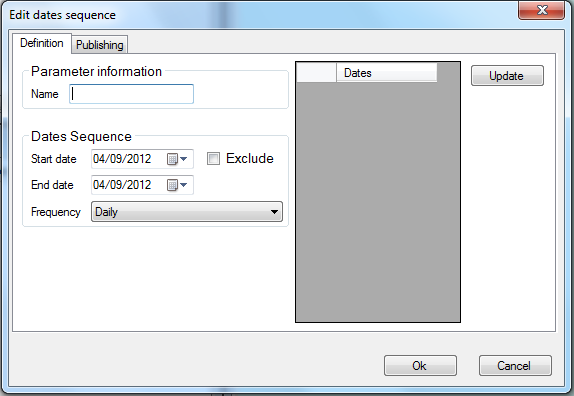
\includegraphics[width=0.8\textwidth]{DG_img}
\centering
\caption{\small{\emph{The Dates Generator editing form.}}}
\label{fig:DG}
\end{figure}

\begin{enumerate}
\item Go to the Parameters \& Functions window
\item Click Add
\item Select Dates Generator and click Ok
\end{enumerate}
As shown Figure~\ref{fig:DG}, it is possible to set the start date and the end date setting also the desidered interval between each date entry (between these options: Daily, Weekly, Bi-Weekly, Montly, Three Months, Six Months, and Year).


%The \textbf{export} checkbox is an adavenced property used to define alternative user %interfaces  (see the fairmat help for more information about that).


In order to edit a previously defined  vector  you'll have to follow a different procedure:
\begin{enumerate}
\item Go to the Parameters \& Functions window.
\item Right click on the vector and select the \textbf{Dates Generator} option.
\item Set the start date, the ending date and the frequency, then press Ok.
\end{enumerate}
The vector will be populated with all the dates as specified.
\end{document}
